\cleardoublepage
\pagenumbering{arabic}
\setcounter{page}{1} 


\chapter{Introducción}
\label{chapter:introduccion}

\section{Contexto y justificación del trabajo}

Durante el desarrollo de este trabajo de fin de máster (TFM) se ha llevado a cabo una caracterización de las posibles duplicidades génicas presentes en los genomas de diferentes cepas bacterianas entre las especies del grupo ESKAPE no analizadas en estudios previos \textit{(Klebsiella pneumoniae, Acinetobacter baumannii, Pseudomonas aeruginosa} y  \textit{Enterobacter} spp.). Para ello se implementarán diversos módulos y paquetes específicos en los lenguajes de programación Python y R que realizarán de manera automática la búsqueda de las mismas. Con los resultados de la obtenidos, se podrán caracterizar genes específicos relacionados con virulencia o resistencia a antimicrobianos y generar gráficas para su visualización.

La duplicación genética es un proceso que se encuentra tanto en células eucariotas como procariotas y es uno de los tipos de mutación más frecuentes \cite{serres_evolution_2009,zhang_evolution_2003}. Es un mecanismo que genera una o más copias indistinguibles del mismo gen en el genoma celular y que se mantiene a lo largo de la línea evolutiva \cite{lynch_genome-wide_2008, lipinski_high_2011, sanchez-herrero_gene_2020, zhang_evolution_2003}. La ventaja evolutiva que proporciona para las bacterias mantener en sus genomas diferentes copias para el mismo gen viene determinada por que cada una de ellas podría mostrar diferentes patrones de expresión e, incluso, responder ante estímulos diferentes, lo cual dota a las cepas que portan esta variedad de copias de más oportunidades para adaptarse a variaciones fisicoquímicas del medio en el que se encuentran. El aumento de la complejidad genómica que genera esta diversidad funcional, facilita la proliferación de las células ante medios limitantes e incrementa las probabilidades de nuevas mutaciones adaptativas \cite{serres_evolution_2009,zhang_evolution_2003}.

Las bacterias del grupo ESKAPE son especialmente patógenas para los seres humanos ya que presentan en su material genético genes de resistencia a diferentes agentes antimicrobianos, lo que las hace difíciles de combatir en caso de infección \cite{lipinski_high_2011, santajit_mechanisms_2016}. La existencia de cepas patógenas multirresistentes a diferentes antibióticos ha supuesto un problema sanitario que lleva a graves consecuencias en la salud pública \cite{bernabeu_gene_2019,murray_vancomycin-resistant_2000, pendleton_clinical_2013, sanchez-herrero_gene_2020}. La limitación de los grupos científicos para crear nuevos antibióticos efectivos y la rapidez con que estas bacterias evolucionan, hace necesario aumentar los conocimientos alrededor de cómo se interrelacionan los diferentes genes bacterianos al expresarse y favorecer la supervivencia de la bacteria \cite{bernabeu_gene_2019,pendleton_clinical_2013,santajit_mechanisms_2016}.

El estudio de duplicidades génicas en \textit{E. coli}, estafilococos y enterococos ha demostrado un patrón diferenciado de las mismas entre las cepas más virulentas y las que no presentan patogenicidad. Se ha constatado la presencia de un número significativo de genes duplicados en cepas patógenas, respecto a aquellas no patógenas, que no se muestran en cepas inofensivas, lo que sugiere que estos genes podrían favorecer de forma relevante la virulencia de las mismas \cite{bernabeu_gene_2019,sanchez-herrero_gene_2020}.

La duplicación genética en bacterias se produce más frecuentemente por transferencia horizontal genética (HGT) entre diferentes individuos gracias a agentes virales, plásmidos o transposones, que por diferentes mecanismos moleculares naturales que pueden generar duplicaciones en los genomas bacterianos \cite{reams_mechanisms_2015,romero_gene_1997,sanchez-herrero_gene_2020,santajit_mechanisms_2016}. 

Identificar genes duplicados específicos en diferentes cepas patógenas, podría contribuir al estudio de los mecanismos de la virulencia de las mismas ampliando la información ya conocida sobre cómo se regula la expresión genética en las bacterias a estudio \cite{bernabeu_gene_2019,sanchez-herrero_gene_2020}. Por otro lado, si se determinara la codificación por parte de alguno de estos genes duplicados de productos antigénicos, se podrían desarrollar nuevas vacunas o medicamentos más efectivos para hacer frente a las enfermedades provocadas por este tipo de bacterias \cite{bernabeu_gene_2019, serres_evolution_2009}.

Por todo lo mencionado, en este Trabajo de TFM se complementarán los trabajos realizados por \cite{bernabeu_gene_2019} y \cite{sanchez-herrero_gene_2020} desarrollando una herramienta bioinformática capaz de llevar a cabo de manera automatizada todo el proceso de búsqueda e identificación de duplicidades dentro de un genoma dado. Se obtendría como resultado un archivo de datos con toda la información obtenida y una representación gráfica con el fin de facilitar su estudio y comprensión. Estos resultado podrán utilizarse facilmente en estudios de investigación relacionados.

Desarrollar una herramienta bioinformática, compuesta de diversos módulos específicos para cada una de las fases que comprenden el análisis genómico y la búsqueda de duplicidades, permitirá a la comunidad científica avanzar de forma más ágil en la investigación sobre el tema.



\section{Objetivos del Trabajo}

Los objetivos desarrollados a lo largo de este TFM han sido los siguientes:
\begin{itemize}
    \item Desarrollo de herramientas bioinformáticas para el análisis y caracterización de duplicidades genéticas en bacterias.
    \begin{itemize}
        \item Desarrollar funciones de python para el tratamiento y análisis de duplicaciones tanto de secuencias genómicas en bases de datos como ensambladas \textit{de novo} por parte del usuario.
        \item Implementar la generación y representación de resultados para la mejor interpretación y visualización de los datos.
    \end{itemize}
    \item Caracterización de duplicaciones génicas en una selección de cepas bacterianas.
    \begin{itemize}
        \item Selección de cepas del grupo ESKAPE para caracterizar duplicaciones génicas.
        \item Analizar las secuencias genómicas de las cepas seleccionadas y localizar e identificar genes duplicados
    \end{itemize}
\end{itemize}

\section{Enfoque y método seguido}
% Indicar cuáles son las posibles estrategias para llevar a cabo el trabajo e indicar cuál es la estrategia elegida (desarrollar un producto nuevo, adaptar un producto existente, …). Valorar porque esta es la estrategia más apropiada para conseguir los objetivos
A pesar de que ya existen trabajos previos en los cuales se muestran técnicas para el análisis de duplicidades génicas \cite{bernabeu_gene_2019, sanchez-herrero_gene_2020}, estos no presentan un desarrollo de herramientas bioinformáticas que permitan automatizar totalmente el proceso de análisis y posterior interpretación de los resultados. La estrategia que se llevará a cabo en este TFM procurará una única metodología de análisis genómico que permita a la comunidad científica realizar este proceso de una forma más directa. Cada fase del análisis, desde la lectura de los datos hasta la visualización e interpretación de resultados, se englobará en un único proceso, lo que facilitará el uso y difusión de las herramientas generadas.

En primer lugar, se han desarrollado módulos en Python \cite{Rossum_2009} para leer de manera automática la secuencia genómica proporcionada por el usuario y analizar la información indicada. Posteriormente, con la herramienta de análisis de secuencias BLAST+ \cite{madden_blast_2003}, se ha implementado otros módulos para buscar e identificar genes duplicados y generar un archivo de resultados. Los diferentes módulos creados en python se han integrado en una única herramienta que trabajará de manera automática a lo largo de todos los pasos requeridos para completar el análisis.

Finalmente, se ha creado un paquete en R \cite{R_core} para mostrar los resultados de manera interactiva con el programa BioCircos \cite{biocircos} que facilitan su interpretación. Este módulo se ha generado a partir del aportado por \cite{sanchez-herrero_gene_2020} con las modificaciones pertinentes para adaptarlo a nuestras necesidades.

Una vez desarrollada esta versión beta del programa, se ha desarrollado el segundo objetivo y analizado cepas bacterianas reales para generar resultados.


\section{Planificación del Trabajo}

% Descripción de los recursos necesarios para realizar el trabajo, las tareas a realizar y una planificación temporal de cada tarea utilizando un diagrama de Gantt o similar. Esta planificación tendría que marcar cuáles son los hitos parciales de cada una de las PEC.

Los objetivos y tareas realizados se han planteado según los diferentes hitos marcados por el plan docente. Estos hitos corresponden a cada una de las pruebas de evaluación continua (PEC) propuestas a lo largo del periodo estipulado, así como la entrega de la memoria final y la defensa pública del proyecto por medio de una presentación virtual.

La imagen \ref{fig:crono} representa la planificación del TFM. Se ha desglosado cada objetivo en las correspondientes tareas a realizar a lo largo de la línea temporal.

\begin{figure}[h]
	\centering
	\captionsetup{width=0.7\linewidth} 
	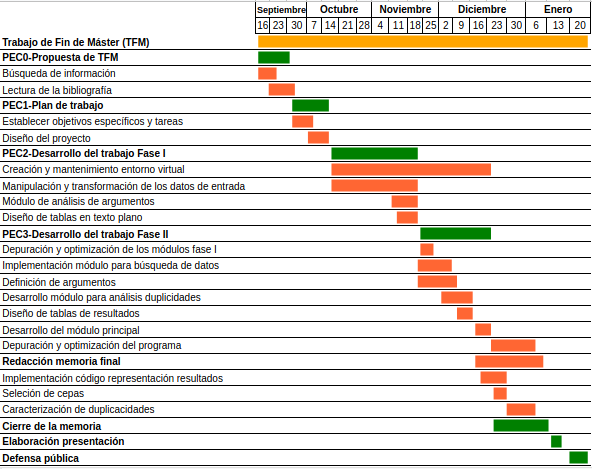
\includegraphics[width=0.7\linewidth]{figs/cronograma.png}
	\caption[Cronograma]{Cronograma detallado de la planificación del trabajo a lo largo de desarrollo del TFM. En verde se representan las entregas de documentación y en naranja las diferentes tareas realizadas.}
	\label{fig:crono}
\end{figure}
A continuación, se presenta un breve resumen de algunas de las tareas realizadas más significativas:

\begin{itemize}
    \item \textbf{Creación de un entorno virtual en Python: }para poder realizar correctamente las tareas de programación, se ha creado un espacio único para el proyecto en el que se albergue las diferentes librerías instaladas. El manejo del programa de instalación \textit{pip} ha sido fundamental para el desarrollo de este entorno. Así como el uso de aplicaciones para el control de versiones como GIT y el trabajo colaborativo en plataformas virtuales como GitHub ha favorecido la fluidez a la hora de realizar correcciones y sugerencias por parte del director de TFM y la comunicación entre ambas partes.
    
    \item \textbf{Desarrollo de módulos básicos: }Se han creado las diferentes funciones necesarias para implementar el módulo para la búsqueda de datos. Estos módulos básicos se han concebido como pequeños fragmentos de código funcionales capaces de realizar las diferentes acciones de manipulación y transformación de los datos proporcionados. De esta forma, se obtendrán objetos que puedan ser utilizados en el módulo principal. Se han utilizado herramientas en BioPython profundizando en la documentación proporcionada para cada función y adaptándolas a nuestras necesidades para la creación de los nuevos programas.
    
    \item \textbf{Transformación de la información a texto plano: }mediante los programas Pandas y Numpy, se han manipulado los archivos de anotación genómicos (e.g. genbank, GTF, GFF) para crear objetos de python con la estructura adecuada para generar tablas y poder volcarlas como texto plano y visualizarlas, por ejemplo, en un procesador de hojas de cálculo. Estas tablas se han utilizado posteriormente para analizar las duplicidades génicas de los genomas estudiados.
    
    \item \textbf{Depuración de los módulos creados: }durante la primera fase del proyecto, se generaron una serie de módulos que debían ser depurados para su correcto funcionamiento. El seguimiento de errores de programación y su resolución han llevado un tiempo necesario para que el funcionamiento de los siguientes módulos asociados fuera correcto. Se ha implementado el programa de forma que sea muy flexible en cuanto al tipo de información proporcionada por el usuario.
    
    \item \textbf{Definición de argumentos: }para desarrollar una herramienta versátil y de fácil manejo por parte del usuario, se debe ofrecer un amplio rango de posibilidades que faciliten su uso sea cuál sea el tipo de archivo que se utilice para la búsqueda de duplicidades. Así, se han previsto distintos escenarios para definir los argumentos posibles y generar los resultados en una única línea de comandos en la consola LINUX.
    
    \item \textbf{Diseño de tablas de resultados: }mediante los programas Pandas y Numpy se han definido los archivos de texto plano para formatear las tablas con los resultados obtenidos.
    
    \item \textbf{Desarrollo del módulo principal: }Para posibilitar la búsqueda de duplicidades en solo una línea de comando en la terminal, todos los módulos programados previamente deben relacionarse entre sí para poder funcionar como un conjunto. Este módulo principal recogerá los argumentos proporcionados por el usuario y, en base a ello, utilizará unas funciones u otras para generar el archivo de resultados.
    
    \item \textbf{Implementación del código para la representación de resultados: }Implementación del módulo en R que permitirá representar los resultados. Con el paquete BioCircos se ha diseñado un script adaptado a las peculiaridades de los datos generados por el programa en python para generar gráficos representativos del genoma estudiado y los diferentes grupos de duplicados relacionados entre sí.
\end{itemize}












\section{Breve sumario de productos obtenidos}
% No hay que entrar en detalle: la descripción detallada se hará en el resto de capítulos. 

Durante el periodo de realización del TFM se han entregado los siguientes documentos:

\begin{itemize}
    \item Propuesta de TFM.
    \item Pruebas de evaluación contínua:
    \begin{itemize}
        \item Definición de los contenidos del trabajo.
        \item Plan de trabajo.
        \item Informes de seguimiento
    \end{itemize}
\end{itemize}

A estos documentos, se deben añadir la presente memoria y la presentación y defensa del TFM. Finalmente, se realizará un informe de autoevaluación que también será entregado con el resto de documentación.

Además de estos documentos, se han obtenido los siguientes productos:

\begin{itemize}
    \item Secuencias de comandos (scripts) de los módulos en python.
    \item Script del programa en R.
    \item Tablas de anotación y gráficos de las duplicidades génicas de las cepas seleccionadas.
    \item Repositorio público en github con todos los scripts desarrollados, documentación y resultados generados. ******incluir link cuando esté todo listo****
\end{itemize}

\section{Breve descripción de los otros capítulos de la memoria}
El capítulo \ref{chapter: desarrollo} se ha dedicado a explicar detalladamente cada módulo desarrollado y su funcionamiento. Cada una de las secciones del capítulo corresponde a las diferentes fases del proceso, desde la entrada de datos hasta la generación de resultados y su representación gráfica.

El capítulo \ref{chapter: analisis} describe el uso de las herramientas creadas para el análisis de duplicidades en cepas bacterianas seleccionadas. 

El apédice \ref{apA} contiene información sobre los requerimientos necesarios para utilizar los módulos implementados. Se resume brevemente los programas complementarios que se deben instalar y los enlaces al repositorio en github para la descarga de los scripts completos.

Por último, el apéndice \ref{apB} incluye los resultados obtenidos en el análisis de las cepas seleccionadas.